% Cover
\imprimircapa

% False cover sheet
%\imprimirfalsafolhaderosto

% Cover sheet
\imprimirfolhaderosto

% Card Catalog
\begin{fichacatalografica}
	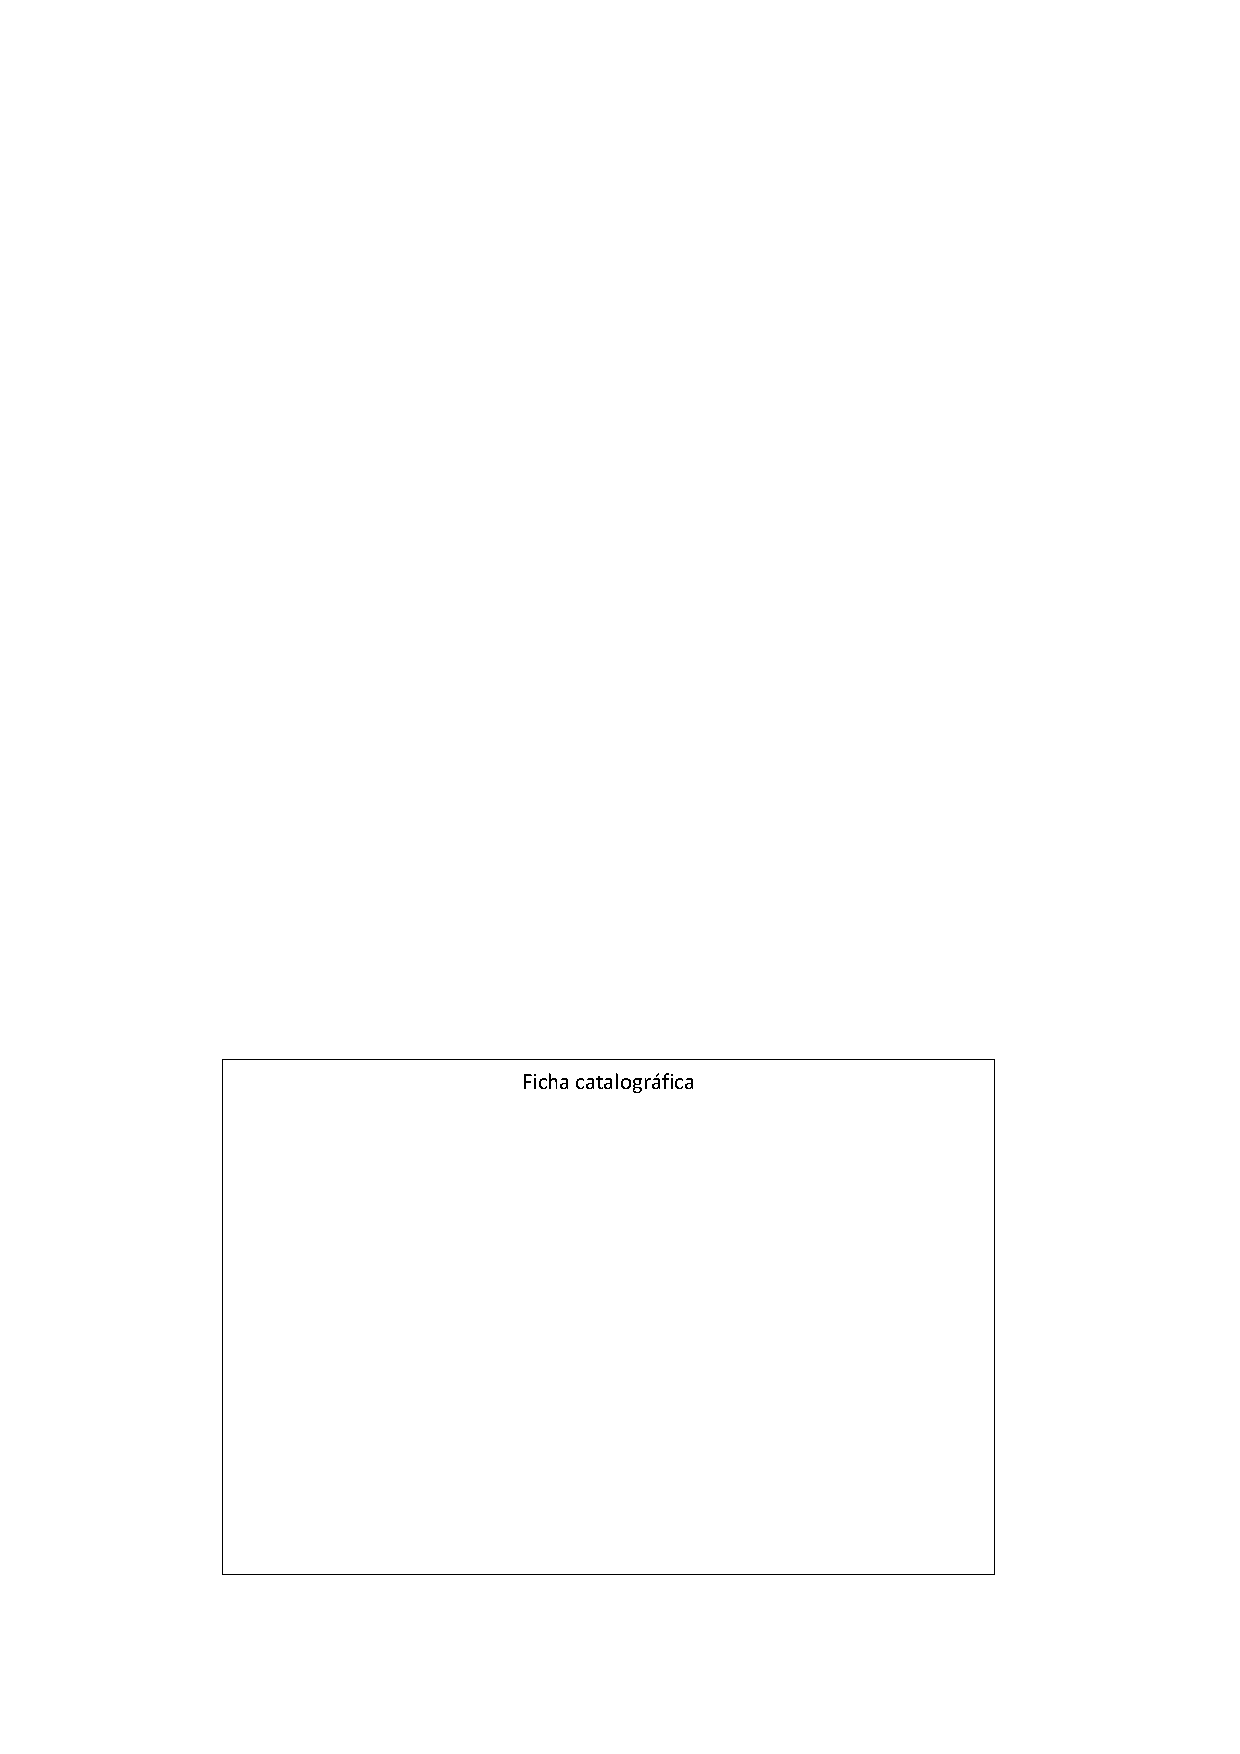
\includepdf{card-catalog.pdf}
\end{fichacatalografica}

% Approval sheet
%\begin{folhadeaprovacao}
%	
%	\begin{center}
%		{\ABNTEXchapterfont\large\imprimirautor}
%		
%		\vspace*{\fill}\vspace*{\fill}
%		\begin{center}
%			\ABNTEXchapterfont\bfseries\Large\imprimirtitulo
%		\end{center}
%		\vspace*{\fill}
%		
%		\hspace{.45\textwidth}
%		\begin{minipage}{.5\textwidth}
%			\imprimirpreambulo
%		\end{minipage}%
%		\vspace*{\fill}
%	\end{center}
%	
%	%Trabalho aprovado. \imprimirlocal, 31 de dezembro de 2020:
%	
%	\assinatura{\textbf{\imprimirorientador} \\ Orientador} 
%	\assinatura{\textbf{\imprimircoorientador} \\ Coorientador} 
%	\assinatura{\textbf{A} \\ Convidado 1}
%	\assinatura{\textbf{B} \\ Convidado 2}
%	
%	\begin{center}
%		\vspace*{0.5cm}
%		{\large\imprimirlocal}
%		\par
%		{\large\imprimirdata}
%		\vspace*{1cm}
%	\end{center}
%	
%\end{folhadeaprovacao}

% Abstract - Portuguese
\setlength{\absparsep}{18pt} % Spacing
\begin{resumo}
	A mudança de paradigma na indústria referente às recentes modificações em relação às tecnologias de manufatura é chamada de Indústria 4.0 (I4.0). Nesse novo conceito, redes inteligentes de máquinas e processos para indústria com o respaldo de Tecnologias da Informação e Comunicação (TIC) passam a proporcionar um alto nível de automação e intercâmbio de informações entre equipamentos, produtos e demais atores em um ambiente de manufatura.
	Este trabalho aborda uma proposta de desenvolvimento dos detalhes do Modelo de Arquitetura de Referência para a Indústria 4.0 (RAMI4.0), especificamente por meio da introdução do conceito de Memória Digital do Produto (MDP) de forma a se aperfeiçoar a elaboração dessa arquitetura, proporcionando mais robustez ao modelo para uma futura adoção generalizada por parte de empresas por todo o mundo.
	O estudo aborda uma nova estrutura de compartilhamento da MDP do ativo por meio de \textit{Web Services} ao longo da cadeia de suprimentos (CS). Três ativos são analisados: O servidor de informações (produto), o cliente que consome as informações (cada elo da CS) e as descrições dos serviços (contidas no repositório).
	A proposta de estrutura é tratada com base no RAMI4.0 e visa propiciar o surgimento de novos cenários de criação de valor no contexto da I4.0 e incentivar a geração de novos modelos de negócio baseado em dados.
	
	\vspace{\onelineskip}
	
	\noindent
	\textbf{Palavras-chave}: Indústria 4.0. RAMI4.0. Memória digital do produto. Arquitetura orientada a serviços (SOA). Cadeia de suprimentos.
\end{resumo}

% Abstract - English
\begin{resumo}[Abstract]
	\begin{otherlanguage*}{english}
		The paradigm shift in the industry regarding the recent changes in manufacturing technologies is called Industry 4.0 (I4.0). In this new concept, intelligent networks of machines and processes for industry with the support of Information and Communication Technologies (ICT) start to provide a high level of automation and exchange of information between equipment, products and other actors in a manufacturing environment.
		This work addresses a proposal to develop the details of the Reference Architectural Model Industrie 4.0 (RAMI4.0), specifically by introducing the concept of Digital Product Memory in order to improve the elaboration of this architecture, providing more robustness to the model for future widespread adoption by companies worldwide.
		This study addresses a new structure for sharing the Digital Product Memory throughout the supply chain by means of Web Services. Three assets are analyzed: The information server (product), the client that consumes the information (each partner in the supply chain) and the service descriptions (stored in the repository).
		The proposed structure is based on the RAMI4.0 and aims to provide means for the emergence of new scenarios for value creation in the context of I4.0 and encourage the creation of new data-driven business models.
		
		\vspace{\onelineskip}

		\noindent 
		\textbf{Keywords}: Industry 4.0. RAMI4.0. Digital product memory. Service-oriented architecture (SOA). Supply chain. 
	\end{otherlanguage*}
\end{resumo}

% List of illustrations
\pdfbookmark[0]{\listfigurename}{lof}
\listoffigures*
\cleardoublepage

% List of tables
\pdfbookmark[0]{\listtablename}{lot}
\listoftables*
\cleardoublepage

% List of abbreviations and acronyms
\begin{siglas}
	\item[AAS] \textit{Asset Administration Shell} (Casca Administrativa do Ativo)
	\item[API] \textit{Application Programming Interface} (Interface de Programação de Aplicação)
	\item[BD] Banco de Dados
	\item[BI] \textit{Business Intelligence} (Inteligência Empresarial)
	\item[C4.0] Componente 4.0
	\item[CS] Cadeia de Suprimentos
	\item[CV] Cadeia de Valor
	\item[CVP] Ciclo de Vida do Produto
	\item[GCVP] Gestão do Ciclo de Vida do Produto
	\item[GI] Gestão da Informação
	\item[I4.0] Indústria 4.0
	\item[IIoT] \textit{Industrial Internet of Things} (Internet das Coisas Industrial)
	\item[IoT] \textit{Internet of Things} (Internet das Coisas)
	\item[LGPD] Lei Geral de Proteção de Dados
	\item[MDP] Memória Digital do Produto
	\item[MFG] \textit{Mark Flow Graph}
	\item[OEE] \textit{Overall Equipment Effectivences} (Eficiência Global do Equipamento)
	\item[OSI] \textit{Open System Interconnection} (Interconexão Aberta de Sistemas)
	\item[PFS] \textit{Production Flow Schema} (Esquema de Fluxo de Produção)
	\item[QoS] \textit{Quality of Service} (Qualidade de Serviço)
	\item[RAMI4.0] \textit{Reference Architectural Model Industrie 4.0} (Modelo de Arquitetura de Referência para a Indústria 4.0)
	\item[REST] \textit{Representational State Transfer} (Transferência Representacional de Estado)
	\item[RFID] (\textit{Radio-Frequency IDentification}) (Identificação por Radiofrequência)
	\item[SOA] \textit{Service Oriented Architecture} (Arquitetura Orientada a Serviços)
	\item[SED] Sistemas a eventos discretos
	\item[TIC] Tecnologia da Informação e Comunicação
  	\item[UUID] \textit{Universal Unique IDentifier} (Identificador Único Universal)
  	\item[WS] \textit{Web Service} (Serviço Web)
  	\item[WSD] \textit{Web Services Description} (Descrição do Serviço Web)
  	\item[WSDL] \textit{Web Services Description Language} (Linguagem de Descrição de Serviços Web)
\end{siglas}

% Summary
\pdfbookmark[0]{\contentsname}{toc}
\tableofcontents*
\cleardoublepage
